% ---------------------------------------------------
% ----- Chapters of the template
% ----- for Bachelor-, Master thesis and class papers
% ---------------------------------------------------
%  Created by C. Müller-Birn on 2012-08-17, CC-BY-SA 3.0.
%  Freie Universität Berlin, Institute of Computer Science, Human Centered Computing. 
%
% TODO remove 2 - to use auto numbering
\chapter{User research and analysis}
\label{chap:research}


% Due to the limited size of the user group, the goal was not to gain <TODO> with high diversity of their demographics, but to have information saturation from fewer but more valuable insights into peolpe with diffrent workflows.

Cites:
\begin{itemize}
  \item \cite{Ross:2016} why companies dont conduct user research
\end{itemize}

Over ten years after the publication of Tomer Sharon's book ''It's our Research'', the listing of qoutes in the introduction about user research in software companies still feel as relevant as ever.
\\
''Yeah, but this study will delay our launch date.'', ''Yeah, but we can't learn much from only five participants.'', ''Yeah, but research sounds so academic.'' \cite[p. 4]{Sharon:2012mk} are only some of the statements that according to Sharon are often heard in software companies when discussing if UX research should be conducted.
\\
The common pressure from different stakeholders often leads to quick implementation of features and workflows without first investing time to figure the user's needs out, which may be faster in the beginning, but can badly impact the user's acceptance of the product due to cumbersome and slow workflows,
in the worst case leading to the user not using the product anymore.

To counteract this, it is crucial to conduct and evaluate user research methods, which is what I did for the development of the UI builder.

A starting point for qualitative user research is to define the goals through the help of the SMART criteria, which provide guidelines and formulated goals during research.

For the project, I defined the SMART criteria as following:

\begin{itemize}
  \item \textbf{specfic} - improve the workflow of users modifying dynamic resources for the Purple Experience.
  \item \textbf{measurable} - interviews after testing period concerning working speed, confidence and <TODO Spaß?> when editing resources, automated user tracking
  \item \textbf{assignable} - research and implementation will mostly be conducted by me, with input from CTO \& product owner, connections to external users through customer service team
  \item \textbf{realistic} - new software platform which reacts quicker, prvides more safety regarding errors and is scalable and extensible in the future. Limiting factors are time (as I only have three months for the first phase, including writinh this thesis)
  \item \textbf{time-related} - the new software should have at least the same feature set and be usable by company-internal users until the end of 2022
\end{itemize}

\section{Identifying and categorizing users and user groups}
\label{sec:user-groups}
In order to effectively design and implement the UI editor, it is crucial to understand the needs and preferences of the various users and user groups who will be using the tool.
Therefore, the first step in the user research process was to identify and categorize the different users and user groups who will be using the editor.

In a later chapter (\ref{sec:personas}), I'll build concrete Personas for the different user groups utilizing the information gained from the interviews.
\\
Because we already have existing users that work with the previous editors and other tools from the ecosystem, it was relatively easy to collect a list of internal and extneral users, which either I personally knew or I could write a short message asking about if and how they use existing tools and modify dynamic resources.
I see that this won't be as easy when dealing with a larger user base or primary external customers, when this first step probably requires more effort to collect a user overview upfront.
\\
With a list of many of the users, I started grouping them to understand the characteristics and needs of each user group, through which can ensure that the UI editor is tailored to their specific requirements and can be used effectively by all users\footnote{When I refer to ''all users'', I mean the group of users that are expected to work with the tool. There is an expected technical and domain specific base knowledge that the Editor won't cover}.
\\
I derived the follwoing commomn factors from the users, which made the communication and categorization a lot easier.

\begin{itemize}
  \item \textbf{quantitative usage} There were users who relied on the tools for most of their work, while others like the external customers accessed the tool a few times a year.
  \item \textbf{common tasks} I roughly categorized the common tasks into three groups:
    \subitem \textbf{Heavy configuration} Mostly internal devs used the tools to build new apps and websites from scratch (or derived from exisiting apps), making many modifications, from structural changes to the seperate views, menus, data sources and more, over styling and translating messages to diffrent languages.
    \subitem \textbf{Moderate configuration} Project devs and customer support people copy resources from existing apps and adapt them for new brands, which often includes changing colors and logos, adapting texts or switching authentification flows.
    \subitem \textbf{Small changes} External customers often only use the tools to exchange some ads, translations or logos, which affects a small set of files.
  \item \textbf{expertise} 
  %<kann man bei schlechter software gut erkennen, leute mit viel erfahrung checken sachen, aber ist für neue nicht intutitiv>
    \subitem \textbf{Technical} Depending on the area of education and working time in the web development industry, the expertise about web technologies, languages like CSS and JSON and often also intuition differs between users.
    \subitem \textbf{Domain- and Platform Specific} There is a lot of vocabulary, functionality of the Purple Experience and other systems as well as permutations of configurations that users learn with time.
\end{itemize}

% ... more
\section{Qualitative user resarch}

\begin{itemize}
  \item mix interview / moderated observation
  \item experiences, outcomes, what went good and bad
\end{itemize}

\subsection{Interview}

TODO interview preparation and conduction

\subsection{Moderated observation}

TODO prep and conducting

\section{Quantitaive user research}

Not used survey / questionaire -> lay down reasons why not necessary in that situation

Tracking of user behaviours

- on site using G analytics \& (the other GDPR compliant tracking tool name??)
- using server logs to understand usage patterns

\section{Process and vizualize the outcomes of the initial user research phase}

\subsection{2x2 Opportunity Matrix}

This two-dimensional vizualization of a set of proposed features prooved helpful when prioritizing tasks with other stakeholders,
as it shows the (approximated) cost of implementation as well as the value the feature can have for users.

The matrix I used is a slightly modified adaption from \cite[p. 181]{LearnHCI:2020ys}, replaced the term ''idea originality'' on the x-axis with ''Value''.

\begin{figure}[ht]
	\centering
  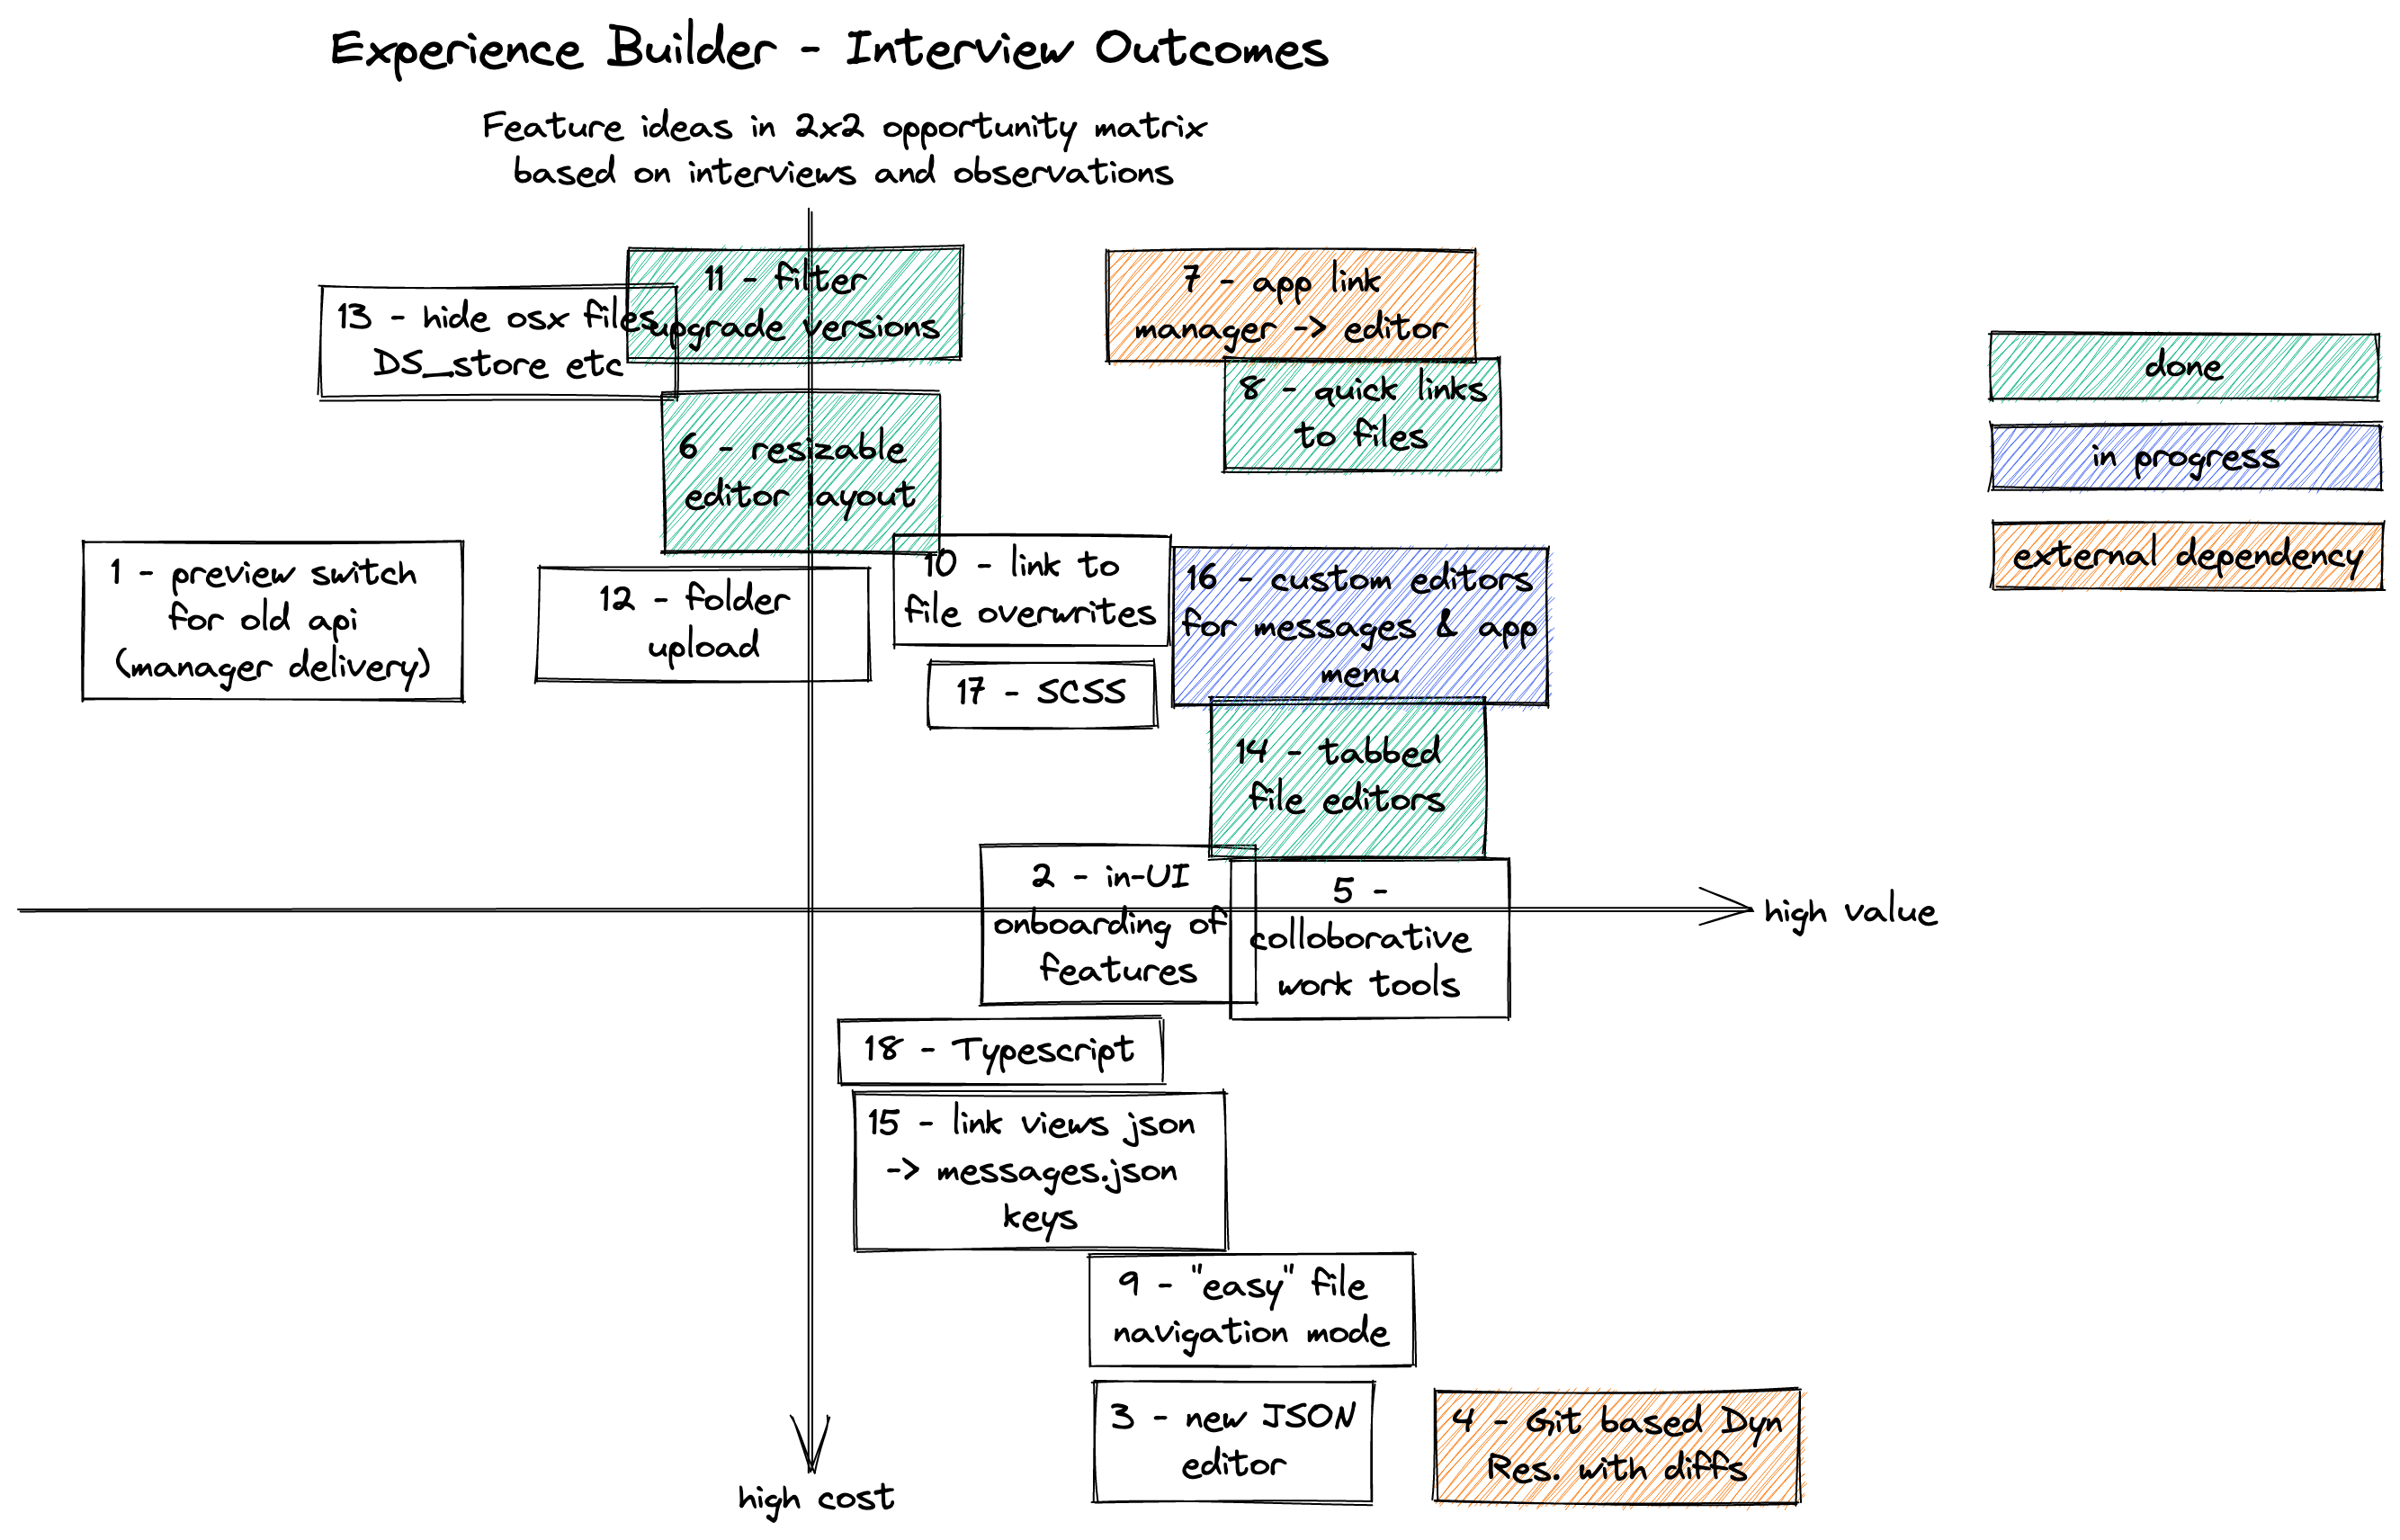
\includegraphics[width=\textwidth]{pics/feature_cost_matrix.excalidraw.png}
	\caption{2x2 Opportunity Matrix during the early phases of development}
	\label{fig:opportunitymatrix}
\end{figure}


\section{Building Personas}
\label{sec:personas}

Personas are descriptions of fictional users of the product, incorporating assumptions and optinally data for a user group.
They aim to give developers and designers more context and depict real potential users, which makes it easier for a developer to empathize with the user.
The following three Role-based Personas are derived from \ref{sec:user-groups} and the outcomes of the interviews, based on the description of Personas in \cite[pp. 403-405]{Interactiondesign:2019ys}
\\
\hrule
% Persona 1
\subsection{John - Purple Expeirence Product Developer}
\subsubsection{Background and Skills}
John (34) is a senior Angular Web Developer at Sprylab, working there for two years. He was born in Berlin and lives in Lichterfelde with his wife and mostly works from home. He is passionate about Angular, Typescript and Developer Experience in general, studied Computer Science at the Beuth Hochschule and hosts Angular conferences.
\\
\subsubsection{Goals and work with the Editor}
\begin{itemize}
  \item Test newly developed features and the related configurations
  \item Configure test apps for development and QA purposes
  \item Support in case Project Developers like <TODO> encounter problems
  \item John works with the editor multiple times a week
\end{itemize}

\hrule
% Persona 2
\subsection{Steffi - Project Developer}
\subsubsection{Background and Skills}
Steffi (23) studies media informatics and works as a working student at Sprylab since a year. This is her first job in the industry and she is learning new things every day. Her skills include writing CSS and understanding modern web technologies, but she still struggles using native and custom debugging tools if something goes wrong.  
\\
\subsubsection{Goals and work with the Editor}
\begin{itemize}
  \item Configure new apps based on existing templates and adapt them to customer's requirements
  \item Add new components or change data sources for existing apps
  \item Add custom HTML pages or Javascript snippets to intergrate external services
  \item Change styles, color schemas or icons when a customer has a rebranding
  \item Steffi uses the editor as a primary tool for her work
\end{itemize}

\hrule
% Persona 2
\subsection{Karsten - IT department at a publishing house}
\subsubsection{Background and Skills}
Karsten (46) worked in the publishing industry for 20 years, but only during the last years his company, aga magazine publisher, tries to catch up with the digital development and trends. He is still struggling with his role and is thankful for every trick or tool that makes his life managing the digital products easier.
\\
\subsubsection{Goals and work with the Editor}
\begin{itemize}
  \item Exchange logos and colors when the magazines he supervies get a redesign
  \item Add new ads to different views when a new campaign starts
  \item Manage URLs to external sites when they change
  \item Karsten uses the Editor once a month on average
\end{itemize}
